% !TEX root = task-3-12-2.tex
% Editable task bank. Append new BankTask blocks at the end of the document.
\documentclass[12pt,a4paper]{article}
\usepackage{physics-textbook}
\usepackage{graphicx,needspace}
\usetikzlibrary{decorations.pathmorphing}
\newif\ifShowSolutions
\ifdefined\TutorEdition
  \ShowSolutionstrue
\else
  \ShowSolutionsfalse % Change to \ShowSolutionstrue to display solutions.
\fi
\newcounter{banktask}
\newsavebox{\BankTaskBox}
\newcommand{\BankTaskContent}[3]{%
  \noindent\textbf{\thebanktask.}\quad #2\par
  \ifShowSolutions
    \Needspace{50mm}% Keep the solution heading with its opening text or diagram.
    #3\par
    \ifdefined\TutorEdition
      \ifcsname TutorSource#1\endcsname
        \nopagebreak\smallskip{\small\csname TutorSource#1\endcsname\par}%
      \fi
    \fi
  \fi
}
\newcommand{\BankTask}[3]{%
  \refstepcounter{banktask}\par\medskip
  \sbox{\BankTaskBox}{\begin{minipage}{\linewidth}%
    \BankTaskContent{#1}{#2}{#3}\end{minipage}}%
  \ifdim\dimexpr\ht\BankTaskBox+\dp\BankTaskBox\relax>\dimexpr\textheight-20mm\relax
    \Needspace{35mm}\BankTaskContent{#1}{#2}{#3}%
  \else
    \Needspace{\dimexpr\ht\BankTaskBox+\dp\BankTaskBox\relax}%
    \noindent\usebox{\BankTaskBox}\par
  \fi
  \medskip
}
\begin{document}
\BookSubsection{3.12.2}{Закон Ома для полной цепи}


% Source sdamgia-10223: https://phys-ege.sdamgia.ru/problem?id=10223
\BankTask{sdamgia-10223}{
При подключении куска проволоки к полюсам батареи через нее течет ток силой $0{,}5\,\text{А}$. Этот кусок проволоки сложили пополам, место сгиба разрезали. Затем разрезали каждый получившийся короткий провод на две равные части, зачистили концы и присоединили все эти части к полюсам батареи параллельно. Найдите силу тока, которая будет течь через батарею в этом случае. Внутреннее сопротивление батареи очень мало.
}{
\smallskip\noindent\textbf{Решение}\par
Сопротивление длинного однородного проводника обратно пропорционально площади его сечения: $R= \frac{\rho l}{S} .$ Всю проволоку сопротивлением R разрезали на $4$ равные части сопротивлением $R/4$ каждая. Общее сопротивление такой цепи при параллельном соединении будет равно $R_0=R/16.$ Тогда по закону Ома в цепи будет течь ток, в $16$ раз больший первоначального $I=16I_0=8\,\text{А}.$

Ответ: $8$.
}

% Source sdamgia-3194: https://phys-ege.sdamgia.ru/problem?id=3194
\BankTask{sdamgia-3194}{
Резистор с сопротивлением R подключен к источнику тока с внутренним сопротивлением r. Сила тока в цепи равна I. Чему равны ЭДС источника и напряжение на его выводах? Установите соответствие между физическими величинами и выражениями для них.

ФИЗИЧЕСКАЯ ВЕЛИЧИНА

А)  ЭДС источника
Б)  Напряжение на выводах источника

ВЫРАЖЕНИЕ ДЛЯ НЕЕ

$1$)  Ir
$2$)  IR
$3$)  $I ( R + r )$
$4$)  $IR ^2 /r\;$

\begin{center}\begin{tabular}{|c|c|}\hline
A&Б\\\hline
&\\\hline
\end{tabular}\end{center}
}{
\smallskip\noindent\textbf{Решение}\par
Согласно закону Ома для полной цепи, сила тока связана с ЭДС источника, сопротивлением источника и сопротивлением нагрузки соотношением $I= \frac{\mathcal{E}}{R + r} .$ Следовательно, ЭДС источника равна $\mathcal{E} =I ( R + r )$ (А  — $3$). Напряжение на выводах источника равно напряжению на резисторе, которое, в свою очередь, пропорционально произведению силы тока, текущего через него, и сопротивления $U=IR$ (Б  — $2$).

Ответ: $32$.
}

% Source sdamgia-28126: https://phys-ege.sdamgia.ru/problem?id=28126
\BankTask{sdamgia-28126}{
Необходимо собрать экспериментальную установку и определить с ее помощью внутреннее сопротивление аккумуляторной батареи. Для этого школьник взял аккумулятор, ключ, соединительные провода и реостат. Какие двапредмета из приведенного ниже перечня оборудования необходимо дополнительно использовать для проведения этого эксперимента?

$1$.  Резистор.
$2$.  Конденсатор.
$3$.  Секундомер.
$4$.  Амперметр.
$5$.  Вольтметр.
}{
\smallskip\noindent\textbf{Решение}\par
Для определения внутреннего сопротивления аккумулятора применяем закон Ома для полной цепи $I= \frac{\varepsilon}{R + r}$ и закон Ома для участка цепи $I= \frac{U}{R} ,$ откуда $r= \frac{\varepsilon - U}{I} .$ Следовательно, для определения внутреннего сопротивления аккумулятора потребуются вольтметр и амперметр  — $4$, $5$.

Ответ: $45$.
}

% Source sdamgia-4420: https://phys-ege.sdamgia.ru/problem?id=4420
\BankTask{sdamgia-4420}{
Идеальный амперметр и три резистора сопротивлением $R=2$ Ом, $2R$ и $3R$ включены последовательно в электрическую цепь, содержащую источник с $\,\text{ЭДС},$ равной $5$ В, и внутренним сопротивлением $r=8$ Ом. Каковы показания амперметра? (Ответ дайте в амперах.)
}{
\smallskip\noindent\textbf{Решение}\par
Идеальный амперметр не имеет сопротивления. Согласно закону Ома для полной цепи, сила тока в описанной в условии задачи цепи (как раз то, что показывает амперметр) равна: 

\[I= \frac{\mathcal{E}}{r + ( R + 2R + 3R )} = \frac{\mathcal{E}}{r + 6R} = \frac{5\,\text{В}}{8\,\text{Ом} + 6 \cdot 2\,\text{Ом}} =0{,}25\,\text{А}.\]

Ответ: $0{,}25$.
}

% Source sdamgia-8527: https://phys-ege.sdamgia.ru/problem?id=8527
\BankTask{sdamgia-8527}{
Резистор с сопротивлением R подключают к источнику тока с ЭДС $\mathcal{E}_1$ и внутренним сопротивлением $r_1.$ Если подключить этот резистор к источнику тока с ЭДС $\mathcal{E}_2 = 2\mathcal{E}_1$ и внутренним сопротивлением $r_2= r_1,$ то во сколько раз увеличится мощность, выделяющаяся в этом резисторе?
}{
\smallskip\noindent\textbf{Решение}\par
Согласно закону Ома для полной цепи сила тока, текущего через резистор, равна $I= \frac{\mathcal{E}}{R + r} .$ Следовательно, мощность, выделяющаяся в резисторе: $\,\text{Р}=I ^2 R= \frac{\mathcal{E} ^2 R}{( R + r ) ^2} .$ Таким образом, поскольку $r_2= r_1,$ а $\mathcal{E}_2 = 2\mathcal{E}_1$ заключаем, что выделяемая на резисторе мощность увеличится в $4$ раза. Обратите внимание, что зависимость данной величины от внутреннего сопротивления источника менее тривиальна.

Ответ: $4$.
}

% Source sdamgia-19796: https://phys-ege.sdamgia.ru/problem?id=19796
\BankTask{sdamgia-19796}{
Электрическая цепь состоит из последовательно соединенных батареи с ЭДС $12\,\text{В}$ и внутренним сопротивлением $1\,\text{Ом}$, резистора сопротивлением $3\,\text{Ом}$, незаряженного конденсатора и разомкнутого ключа. Ключ замкнули, и после этого оказалось, что в некоторый момент времени напряжение на конденсаторе равно $4\,\text{В}$. Какая сила тока течет в этот момент в данной электрической цепи? Ответ дайте в амперах.
}{
\smallskip\noindent\textbf{Решение}\par
ЭДС источника равно $\mathcal{E} = IR + Ir + U_{\,\text{к}},$ откуда сила тока через резистор в этот момент времени равна:

\[I = \frac{\mathcal{E} - U_{\,\text{к}}}{R + r} = \frac{12 - 4}{3 + 1} = 2\,\text{А}.\]

Ответ: $2$.
}

% Source sdamgia-51363: https://phys-ege.sdamgia.ru/problem?id=51363
\BankTask{sdamgia-51363}{
К батарее с внутренним сопротивлением $1\,\text{Ом}$ подключили резистор с сопротивлением $24\,\text{Ом}$. При этом сила тока в цепи оказалась равной $0{,}2\,\text{А}$. Чему равна ЭДС батареи? Ответ выразите в вольтах.
}{
\smallskip\noindent\textbf{Решение}\par
Из закона Ома для полной цепи $\mathcal{E} = I ( R + r ) = 0{,}2 \cdot ( 24 + 1 ) = 5\,\text{В}.$

Ответ: $5$.
}

% Source sdamgia-1531: https://phys-ege.sdamgia.ru/problem?id=1531
\BankTask{sdamgia-1531}{
При подключении резистора с неизвестным сопротивлением к источнику тока с ЭДС $10\,\text{В}$ и внутренним сопротивлением $1\,\text{Ом}$ напряжение на выходе источника тока равно $8\,\text{В}$. Чему равна сила тока в цепи? Ответ приведите в амперах.
}{
\smallskip\noindent\textbf{Решение}\par
Согласно закону Ома для полной цепи $I= \frac{\mathcal{E}}{R + r} ,$  по закону Ома для участка цепи $I= \frac{U}{R} .$ Тогда получаем соотношение $\mathcal{E} =Ir + U.$ Отсюда находим силу тока в цепи:

\[I= \frac{\mathcal{E} - U}{r} = \frac{10\,\text{В} - 8\,\text{В}}{1\,\text{Ом}} =2\,\text{А}.\]

Ответ: $2\,\text{А}$.
}

% Source sdamgia-7303: https://phys-ege.sdamgia.ru/problem?id=7303
\BankTask{sdamgia-7303}{
К контактам батарейки с некоторым внутренним сопротивлением подсоединен резистор сопротивлением R, при этом через батарейку течет ток силой I$_{1}$. Параллельно с этим резистором подсоединяют второй такой же резистор, и сила тока, текущего через батарейку, изменяется в $1{,}5$ раза. После этого второй резистор R отсоединяют и подключают его последовательно с первым резистором. В результате через батарейку начинает течь ток силой I$_{3}$. Чему равно отношение I$_{3}$/I$_{1}$?
}{
\smallskip\noindent\textbf{Решение}\par
Запишем закон Ома для полной цепи в трех различных случаях:
$1$.  $I_1= \frac{U}{R + r} ,$ здесь r  — внутреннее сопротивление источника;
$2$.  $I_2= \frac{U}{R_{\,\text{общ}} + r} ,$ с учетом сопротивления при параллельном соединении проводников: $1/R_{\,\text{общ}}=1/R_1 + 1/R_2;$
$3$.  $I_3= \frac{U}{R_{\,\text{общ}} + r} ,$ $R_{\,\text{общ}}=2R$  — сопротивление участка цепи при последовательном соединении резисторов.
Из условия: $I_2=1{,}5I_1$ (ток увеличится, так как уменьшится сопротивление участка цепи). Отсюда находим, что:

$\frac{U}{R/2 + r} = \frac{1{,}5U}{R + r} ,$ откуда $R=2r.$

Найдем теперь отношение $I_3/I_1$:

\[\frac{I_3}{I_1} = \frac{R + r}{2R + r} = \frac{3r}{5r} =0{,}6.\]

Ответ: $0{,}6$.
}

% Source sdamgia-10449: https://phys-ege.sdamgia.ru/problem?id=10449
\BankTask{sdamgia-10449}{
К источнику тока с конечным внутренним сопротивлением и ЭДС $6\,\text{В}$ подключен реостат. Максимальная тепловая мощность, выделяющаяся на реостате, равна $4{,}5$ Вт при промежуточном сопротивлении. Найдите это сопротивление.
}{
\smallskip\noindent\textbf{Решение}\par
По закону Ома для полной цепи сила тока, текущего через реостат, равна $I= \frac{\mathcal{E}}{R + r} .$ А значит, мощность, выделяющаяся на реостате, равна $P=I ^2 R= \frac{\mathcal{E} ^2 R}{( R + r ) ^2} .$
Видно, что при $R arrow 0$ и $R arrow \,\text{бесконечность}$ мощность стремится к нулю. Найдем максимум мощности:

$P'_R=0 \Longleftrightarrow \frac{\mathcal{E} ^2 \cdot ( R + r ) ^2 - \mathcal{E} ^2 R \cdot 2 ( R + r )}{( R + r ) ^{4}} =0 \Longleftrightarrow ( R + r ) - 2R=0 \Longleftrightarrow R=r,$
$P_{\max}= \frac{\mathcal{E} ^2 r}{( r + r ) ^2} = \frac{\mathcal{E} ^2}{4r} .$

По условию $P_{\max}=4{,}5\,\text{Вт},$ значит, $r= \frac{\mathcal{E} ^2}{4P_{\max}} = \frac{6 ^2}{4 \cdot 4{,}5} =2\,\text{Ом}.$
Таким образом, максимальная тепловая мощность будет при сопротивлении реостата $R=r=2\,\text{Ом}.$

Ответ: $2\,\text{Ом}$.
}


% Source 4EAC46: https://ege.fipi.ru/bank/questions.php?search=1&proj=BA1F39653304A5B041B656915DC36B38&qid=4EAC46
\BankTask{4EAC46}{
Исследуется электрическая цепь, собранная по схеме, представленной на рисунке.

Определите формулы, которые можно использовать для расчётов показаний амперметра и вольтметра. Считать измерительные приборы идеальными, а сопротивление реостата полностью введённым в цепь.

\begin{center}
\TaskMatchingColumns[0.48\linewidth]{Показания приборов}{
А) показания амперметра\par
Б) показания вольтметра
}{Формулы}{
1) $\displaystyle\frac{\mathcal E}{R+R_{\text{р}}+r}$\par
2) $\mathcal E(R+R_{\text{р}}+r)$\par
3) $\displaystyle\mathcal E-\frac{\mathcal E R}{R+R_{\text{р}}+r}$\par
4) $\displaystyle\frac{\mathcal E R}{R+R_{\text{р}}+r}$
}

\begin{tabular}{|c|c|}
\hline
А & Б \\
\hline
\phantom{22} & \phantom{22} \\
\hline
\end{tabular}

\begin{tikzpicture}[book diagram,x=0.045cm,y=0.045cm]
\draw (0,0) -- (0,57) -- (12,57);
\draw (12,50) -- (12,64);
\draw (19,44) -- (19,70);
\node[above] at (12,70) {$\mathcal E,r$};
\draw (19,57) -- (45,57);
\draw (59,57) circle (14);
\node at (59,57) {$\mathrm A$};
\draw (73,57) -- (85,57) -- (85,38);
\draw (76,38) rectangle (94,-5);
\node[left] at (73,16) {$R$};
\draw (85,-5) -- (85,-27) -- (58,-27);
\fill (85,51) circle (1.7);
\fill (85,-22) circle (1.7);
\draw (85,51) -- (129,51) -- (129,28);
\draw (129,14) circle (14);
\node at (129,14) {$\mathrm V$};
\draw (129,0) -- (129,-22) -- (85,-22);
\draw (15,-18) rectangle (58,-36);
\node[below] at (36.5,-36) {$R_{\text{р}}$};

\draw (0,0) -- (42,0) -- (42,-6);
\draw[-{book tip}] (42,-6) -- (42,-18);
\end{tikzpicture}
\end{center}
}{
\smallskip\noindent\textbf{Решение от GPT}\par
Идеальный вольтметр не проводит ток, а сопротивление идеального амперметра равно нулю, поэтому $I=\dfrac{\mathcal E}{R+R_{\text{р}}+r}$: А — 1. Вольтметр подключён параллельно резистору $R$ и показывает $U=IR=\dfrac{\mathcal E R}{R+R_{\text{р}}+r}$: Б — 4. Ответ: $14$.
}

% Source 15274C: https://ege.fipi.ru/bank/questions.php?search=1&proj=BA1F39653304A5B041B656915DC36B38&qid=15274C
\BankTask{15274C}{
На рисунке показана цепь постоянного тока. Установите соответствие между физическими величинами и формулами, по которым их можно рассчитать ($\mathcal E$ — ЭДС источника тока, $r$ — внутреннее сопротивление источника тока, $R$ — сопротивление резистора).

\begin{center}
\TaskMatchingColumns[0.55\linewidth]{Физические величины}{
А) сила тока через источник при замкнутом ключе К\par
Б) сила тока через источник при разомкнутом ключе К
}{Формулы}{
1) $\displaystyle\frac{\mathcal E}{r+2R}$\par
2) $\displaystyle\frac{\mathcal E}{2R}$\par
3) $\displaystyle\frac{\mathcal E}{r}$\par
4) $\displaystyle\frac{\mathcal E}{R+r}$
}

\begin{tabular}{|c|c|}
\hline
А & Б \\
\hline
\phantom{22} & \phantom{22} \\
\hline
\end{tabular}

\begin{tikzpicture}[book diagram,x=0.045cm,y=0.045cm]
\draw (0,0) -- (0,44) -- (70,44);
\draw (70,30) -- (70,58);
\draw (77,37) -- (77,51);
\node[above] at (74,60) {$\mathcal E,r$};
\draw (77,44) -- (141,44) -- (141,0) -- (134,0);
\draw (85,-11) rectangle (134,11);
\node at (109.5,0) {$R$};
\draw (85,0) -- (56,0);
\draw (7,-11) rectangle (56,11);
\node at (31.5,0) {$R$};
\draw (7,0) -- (0,0) -- (0,-28) -- (25,-28);
\fill (25,-28) circle (1.5);
\draw (25,-28) -- (44,-39);
\draw (49,-28) -- (70,-28) -- (70,0);
\fill (49,-28) circle (1.5);
\node[below right] at (46,-32) {$\mathrm K$};
\end{tikzpicture}
\end{center}
}{
\smallskip\noindent\textbf{Решение от GPT}\par
При замкнутом ключе левый резистор закорочен, поэтому ток через источник $I_{\text{замк}}=\dfrac{\mathcal E}{R+r}$: А — 4. При разомкнутом ключе оба резистора соединены последовательно, поэтому $I_{\text{разомк}}=\dfrac{\mathcal E}{2R+r}$: Б — 1. Ответ: $41$.
}

% Source 10C527: https://ege.fipi.ru/bank/questions.php?search=1&proj=BA1F39653304A5B041B656915DC36B38&qid=10C527
\BankTask{10C527}{
Электрическая цепь на рисунке состоит из источника постоянного напряжения с ЭДС $\mathcal{E}$ и внутренним сопротивлением $r$ и внешней цепи из двух одинаковых резисторов сопротивлением $R$, включённых параллельно. Установите соответствие между физическими величинами и формулами, по которым их можно рассчитать.

\begin{center}
\TaskMatchingColumns[0.53\linewidth]{Физические величины}{
А) мощность тока, выделяющаяся на одном из резисторов $R$\par
Б) мощность сторонних сил в источнике тока
}{Формулы}{
1) $\displaystyle\frac{\mathcal{E}^2R}{4\left(r+\frac{R}{2}\right)^2}$\par
2) $\displaystyle\frac{\mathcal{E}^2R}{2\left(r+\frac{R}{2}\right)^2}$\par
3) $\displaystyle\frac{\mathcal{E}^2r}{\left(r+\frac{R}{2}\right)^2}$\par
4) $\displaystyle\frac{\mathcal{E}^2}{r+\frac{R}{2}}$
}

\medskip
\begin{tabular}{|c|c|}
\hline
А & Б \\
\hline
\phantom{1} & \phantom{1} \\
\hline
\end{tabular}
\end{center}

\begin{center}
\begin{tikzpicture}[book diagram,x=0.8cm,y=0.8cm]
\draw (0,1.9)--(0,3.5)--(4.6,3.5)--(4.6,2.45);
\draw (0,1.55)--(0,0)--(4.6,0)--(4.6,1.1);
\draw (-0.55,1.9)--(0.55,1.9);
\draw (-0.3,1.55)--(0.3,1.55);
\node[left] at (-0.55,2.35) {$\mathcal{E},r$};
\draw (2.3,3.5)--(2.3,2.45);
\draw (1.975,1.1) rectangle (2.625,2.45);
\draw (2.3,1.1)--(2.3,0);
\node[right] at (2.65,1.775) {$R$};
\draw (4.275,1.1) rectangle (4.925,2.45);
\node[right] at (4.95,1.775) {$R$};
\fill (2.3,3.5) circle (1.5pt);
\fill (2.3,0) circle (1.5pt);
\end{tikzpicture}
\end{center}
}{
\smallskip\noindent\textbf{Решение от GPT}\par
Сопротивление внешней цепи равно $R/2$, поэтому ток через источник $I=\mathcal{E}/(r+R/2)$. Через каждый резистор течёт ток $I/2$, и мощность одного резистора равна $P_R=I^2R/4=\mathcal{E}^2R/[4(r+R/2)^2]$, то есть А — 1. Мощность сторонних сил $P_{\text{ст}}=\mathcal{E}I=\mathcal{E}^2/(r+R/2)$, то есть Б — 4. Ответ: $14$.
}

% Source BB603A: https://ege.fipi.ru/bank/questions.php?search=1&proj=BA1F39653304A5B041B656915DC36B38&qid=BB603A
\BankTask{BB603A}{
Электрическая цепь на рисунке состоит из источника постоянного напряжения с ЭДС $\mathcal{E}$ и внутренним сопротивлением $r$ и внешней цепи из двух одинаковых резисторов сопротивлением $R$, включённых параллельно. Установите соответствие между физическими величинами и формулами, по которым их можно рассчитать.

\begin{center}
\TaskMatchingColumns[0.53\linewidth]{Физические величины}{
А) мощность тока, выделяющаяся во внешней цепи из двух резисторов $R$\par
Б) мощность тока, выделяющаяся на внутреннем сопротивлении источника тока
}{Формулы}{
1) $\displaystyle\frac{\mathcal{E}^2R}{4\left(r+\frac{R}{2}\right)^2}$\par
2) $\displaystyle\frac{\mathcal{E}^2R}{2\left(r+\frac{R}{2}\right)^2}$\par
3) $\displaystyle\frac{\mathcal{E}^2r}{\left(r+\frac{R}{2}\right)^2}$\par
4) $\displaystyle\frac{\mathcal{E}^2}{r+\frac{R}{2}}$
}

\medskip
\begin{tabular}{|c|c|}
\hline
А & Б \\
\hline
\phantom{1} & \phantom{1} \\
\hline
\end{tabular}
\end{center}

\begin{center}
\begin{tikzpicture}[book diagram,x=0.8cm,y=0.8cm]
\draw (0,1.9)--(0,3.5)--(4.6,3.5)--(4.6,2.45);
\draw (0,1.55)--(0,0)--(4.6,0)--(4.6,1.1);
\draw (-0.55,1.9)--(0.55,1.9);
\draw (-0.3,1.55)--(0.3,1.55);
\node[left] at (-0.55,2.35) {$\mathcal{E},r$};
\draw (2.3,3.5)--(2.3,2.45);
\draw (1.975,1.1) rectangle (2.625,2.45);
\draw (2.3,1.1)--(2.3,0);
\node[right] at (2.65,1.775) {$R$};
\draw (4.275,1.1) rectangle (4.925,2.45);
\node[right] at (4.95,1.775) {$R$};
\fill (2.3,3.5) circle (1.5pt);
\fill (2.3,0) circle (1.5pt);
\end{tikzpicture}
\end{center}
}{
\smallskip\noindent\textbf{Решение от GPT}\par
Эквивалентное сопротивление двух параллельных резисторов равно $R/2$, поэтому $I=\mathcal{E}/(r+R/2)$. Во внешней цепи выделяется мощность $P_{\text{внеш}}=I^2R/2=\mathcal{E}^2R/[2(r+R/2)^2]$, что соответствует формуле 2. На внутреннем сопротивлении выделяется мощность $P_r=I^2r=\mathcal{E}^2r/(r+R/2)^2$, что соответствует формуле 3. Ответ: $23$.
}

% Source DF5187: https://ege.fipi.ru/bank/questions.php?search=1&proj=BA1F39653304A5B041B656915DC36B38&qid=DF5187
\BankTask{DF5187}{
Два резистора с сопротивлениями $R_1$ и $R_2$ подключены к источнику тока с внутренним сопротивлением $r$ (см. рисунок). Напряжение на втором резисторе равно $U_2$. Чему равны напряжение на первом резисторе и ЭДС источника?

Установите соответствие между физическими величинами и формулами, по которым их можно рассчитать.

\begin{center}
\TaskMatchingColumns[0.49\linewidth]{Физические величины}{
А) напряжение на резисторе $R_1$\par
Б) ЭДС источника
}{Формулы}{
1) $\displaystyle U_2\cdot\frac{R_1}{R_2}$\par
2) $\displaystyle U_2\cdot\frac{R_2}{R_1}$\par
3) $\displaystyle\frac{U_2}{R_1}\cdot(R_1+R_2+r)$\par
4) $\displaystyle\frac{U_2}{R_2}\cdot(R_1+R_2+r)$
}

\medskip
\begin{tabular}{|c|c|}
\hline
А & Б \\
\hline
\phantom{1} & \phantom{1} \\
\hline
\end{tabular}
\end{center}

\begin{center}
\begin{tikzpicture}[book diagram,x=0.8cm,y=0.8cm]
\draw (0,1.85)--(0,3.5)--(1.4,3.5);
\draw (1.4,3.15) rectangle (3.1,3.85);
\draw (3.1,3.5)--(4.5,3.5)--(4.5,2.95);
\draw (4.15,1.25) rectangle (4.85,2.95);
\draw (4.5,1.25)--(4.5,0)--(0,0)--(0,1.55);
\draw (-0.55,1.85)--(0.55,1.85);
\draw (-0.3,1.55)--(0.3,1.55);
\node[left] at (-0.55,2.3) {$\mathcal{E},r$};
\node[below] at (2.25,3.12) {$R_1$};
\node[right] at (4.9,2.1) {$R_2$};
\end{tikzpicture}
\end{center}
}{
\smallskip\noindent\textbf{Решение от GPT}\par
При последовательном соединении ток через оба резистора одинаков: $I=U_2/R_2$. Тогда напряжение на первом резисторе $U_1=IR_1=U_2R_1/R_2$, то есть А — 1. По закону Ома для полной цепи $\mathcal{E}=I(R_1+R_2+r)=\dfrac{U_2}{R_2}(R_1+R_2+r)$, то есть Б — 4. Ответ: $14$.
}

% Source D860B0: https://ege.fipi.ru/bank/questions.php?search=1&proj=BA1F39653304A5B041B656915DC36B38&qid=D860B0
\BankTask{D860B0}{
Ученик изучает законы постоянного тока. В его распоряжении имеется пять аналогичных электрических цепей (см. рисунок) с различными источниками и внешними сопротивлениями, характеристики которых указаны в таблице. Какие две цепи необходимо взять ученику для того, чтобы на опыте обнаружить зависимость силы тока, протекающего в цепи, от внутреннего сопротивления источника?

\begin{center}
\begin{tabular}{|c|c|c|c|}
\hline
№ цепи & \shortstack{ЭДС источника\\$\varepsilon$, \(\text{В}\)} & \shortstack{Внутреннее сопротивление\\источника $r$, \(\text{Ом}\)} & \shortstack{Внешнее сопротивление\\$R$, \(\text{Ом}\)} \\
\hline
\(1\) & \(6\) & \(1{,}0\) & \(5\) \\
\hline
\(2\) & \(9\) & \(0{,}5\) & \(8\) \\
\hline
\(3\) & \(8\) & \(1{,}5\) & \(16\) \\
\hline
\(4\) & \(9\) & \(1{,}5\) & \(8\) \\
\hline
\(5\) & \(6\) & \(0{,}5\) & \(16\) \\
\hline
\end{tabular}
\end{center}

\begin{center}
\begin{tikzpicture}[book diagram]
\draw (0,0.82) -- (0,1.4) -- (0.9,1.4);
\draw (0,0.38) -- (0,0.02) -- (0.5,0.02);
\draw (0,0.6) circle (0.22);
\node at (0,0.6) {$\mathrm{A}$};
\draw (0.9,1.08) -- (0.9,1.72);
\draw (1.06,1.25) -- (1.06,1.55);
\draw (1.06,1.4) -- (1.95,1.4) -- (1.95,0.02) -- (1.5,0.02);
\draw (0.5,-0.18) rectangle (1.5,0.22);
\node[above] at (1,0.22) {$R$};
\node[above] at (1.4,1.55) {$\mathcal{E},\,r$};
\end{tikzpicture}
\end{center}
}{
\smallskip\noindent\textbf{Решение от GPT}\par
По закону Ома для полной цепи $I=\dfrac{\varepsilon}{R+r}$. Для исследования зависимости от $r$ необходимо сохранить одинаковыми ЭДС и внешнее сопротивление: у цепей \(2\) и \(4\) $\varepsilon=9\,\text{В}$ и $R=8\,\text{Ом}$, а внутренние сопротивления различаются. Ответ: \(24\).
}

% Source A88c1A: https://ege.fipi.ru/bank/questions.php?search=1&proj=BA1F39653304A5B041B656915DC36B38&qid=A88c1A
\BankTask{A88c1A}{
Необходимо экспериментально обнаружить зависимость силы тока, протекающего в цепи, от ЭДС источника. Какие две электрические цепи, схемы которых приведены на рисунках, следует использовать для такого исследования?

\begin{center}
\begin{tikzpicture}[book diagram]
\begin{scope}
\node at (0.75,1.95) {1)};
\draw (0,0.77) -- (0,1.3) -- (0.72,1.3);
\draw (0,0.33) -- (0,0) -- (0.38,0);
\draw (0,0.55) circle (0.22);
\node at (0,0.55) {$\mathrm{A}$};
\draw (0.72,1.03) -- (0.72,1.57);
\draw (0.86,1.17) -- (0.86,1.43);
\draw (0.86,1.3) -- (1.6,1.3) -- (1.6,0) -- (1.22,0);
\draw (0.38,-0.18) rectangle (1.22,0.18);
\node[above] at (0.8,0.18) {$R$};
\node[above] at (1.17,1.43) {$\mathcal{E},r$};
\end{scope}
\begin{scope}[xshift=2.6cm]
\node at (0.75,1.95) {2)};
\draw (0,0.77) -- (0,1.3) -- (0.72,1.3);
\draw (0,0.33) -- (0,0) -- (0.38,0);
\draw (0,0.55) circle (0.22);
\node at (0,0.55) {$\mathrm{A}$};
\draw (0.72,1.03) -- (0.72,1.57);
\draw (0.86,1.17) -- (0.86,1.43);
\draw (0.86,1.3) -- (1.6,1.3) -- (1.6,0) -- (1.22,0);
\draw (0.38,-0.18) rectangle (1.22,0.18);
\node[above] at (0.8,0.18) {$2R$};
\node[above] at (1.17,1.43) {$2\mathcal{E},r$};
\end{scope}
\begin{scope}[xshift=5.2cm]
\node at (0.75,1.95) {3)};
\draw (0,0.77) -- (0,1.3) -- (0.72,1.3);
\draw (0,0.33) -- (0,0) -- (0.38,0);
\draw (0,0.55) circle (0.22);
\node at (0,0.55) {$\mathrm{A}$};
\draw (0.72,1.03) -- (0.72,1.57);
\draw (0.86,1.17) -- (0.86,1.43);
\draw (0.86,1.3) -- (1.6,1.3) -- (1.6,0) -- (1.22,0);
\draw (0.38,-0.18) rectangle (1.22,0.18);
\node[above] at (0.8,0.18) {$R$};
\node[above] at (1.17,1.43) {$\mathcal{E},2r$};
\end{scope}
\begin{scope}[xshift=7.8cm]
\node at (0.75,1.95) {4)};
\draw (0,0.77) -- (0,1.3) -- (0.72,1.3);
\draw (0,0.33) -- (0,0) -- (0.38,0);
\draw (0,0.55) circle (0.22);
\node at (0,0.55) {$\mathrm{A}$};
\draw (0.72,1.03) -- (0.72,1.57);
\draw (0.86,1.17) -- (0.86,1.43);
\draw (0.86,1.3) -- (1.6,1.3) -- (1.6,0) -- (1.22,0);
\draw (0.38,-0.18) rectangle (1.22,0.18);
\node[above] at (0.8,0.18) {$2R$};
\node[above] at (1.17,1.43) {$2\mathcal{E},2r$};
\end{scope}
\begin{scope}[xshift=10.4cm]
\node at (0.75,1.95) {5)};
\draw (0,0.77) -- (0,1.3) -- (0.72,1.3);
\draw (0,0.33) -- (0,0) -- (0.38,0);
\draw (0,0.55) circle (0.22);
\node at (0,0.55) {$\mathrm{A}$};
\draw (0.72,1.03) -- (0.72,1.57);
\draw (0.86,1.17) -- (0.86,1.43);
\draw (0.86,1.3) -- (1.6,1.3) -- (1.6,0) -- (1.22,0);
\draw (0.38,-0.18) rectangle (1.22,0.18);
\node[above] at (0.8,0.18) {$2R$};
\node[above] at (1.17,1.43) {$\mathcal{E},r$};
\end{scope}
\end{tikzpicture}
\end{center}
}{
\smallskip\noindent\textbf{Решение от GPT}\par
Согласно формуле $I=\dfrac{\mathcal{E}}{R_{\text{внеш}}+r_{\text{внутр}}}$, для проверки зависимости от ЭДС оба сопротивления должны быть одинаковыми. Цепи 2 и 5 имеют внешнее сопротивление $2R$ и внутреннее сопротивление $r$, а их ЭДС равны $2\mathcal{E}$ и $\mathcal{E}$ соответственно. Для цепи 1 нет пары с теми же сопротивлениями и другой ЭДС; цепи 3 и 4 также не имеют таких пар, поскольку их внешние сопротивления различаются. Ответ: 25.
}

% Source 51472: https://phys-ege.sdamgia.ru/problem?id=51472
\BankTask{51472}{
\begin{center}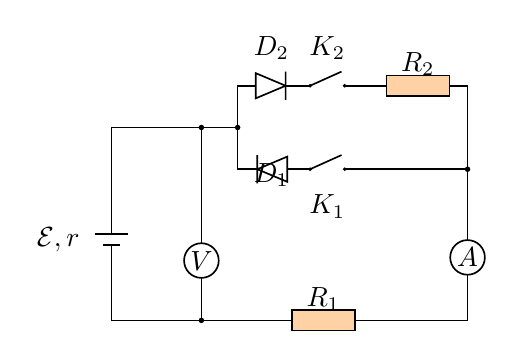
\begin{tikzpicture}[>=stealth,line width=.6pt]

\draw (0,1.1)--(0,2.45)--(1.6,2.45)--(1.6,2.98)--(1.83,2.98)
      (0,.96)--(0,0)--(2.29,0) (3.09,0)--(4.52,0)--(4.52,.58)
      (4.52,1.02)--(4.52,2.98)--(4.29,2.98)
      (1.6,2.45)--(1.6,1.92)--(1.85,1.92) (2.23,1.92)--(2.52,1.92) (2.96,1.92)--(4.52,1.92)
      (2.21,2.98)--(2.52,2.98) (2.96,2.98)--(3.49,2.98)
      (1.14,2.45)--(1.14,.98) (1.14,.54)--(1.14,0);
\fill(1.14,2.45)circle(.035) (1.6,2.45)circle(.035) (1.14,0)circle(.035) (4.52,1.92)circle(.035);
\begin{scope}[shift={(0,1.03)},rotate=-90]\draw(-.07,-.21)--(-.07,.21) (.07,-.11)--(.07,.11);\end{scope}\node[above right] at (0.12,1.03) {$$};\node[left] at (-.28,1.02) {$\mathcal E,r$};\draw (1.14,0.76)circle(.22) node {$V$};\draw (4.52,0.8)circle(.22) node {$A$};\begin{scope}[shift={(2.69,0)},rotate=0]\draw[fill=orange!35] (-.4,-.13) rectangle (.4,.13);\end{scope}\node[above] at (2.69,0) {$R_1$};\begin{scope}[shift={(3.89,2.98)},rotate=0]\draw[fill=orange!35] (-.4,-.13) rectangle (.4,.13);\end{scope}\node[above] at (3.89,2.98) {$R_2$};\begin{scope}[shift={(2.03,2.98)},rotate=0]\draw(-.2,-.16)--(-.2,.16)--(.18,0)--cycle (.18,-.18)--(.18,.18);\end{scope}\node[above] at (2.03,3.18) {$D_2$};\begin{scope}[shift={(2.03,1.92)},rotate=180]\draw(-.2,-.16)--(-.2,.16)--(.18,0)--cycle (.18,-.18)--(.18,.18);\end{scope}\node[below] at (2.03,2.12) {$D_1$};\begin{scope}[shift={(2.74,2.98)},rotate=0]\draw(-.22,0)--(.18,.18);\fill(-.22,0)circle(.025) (.22,0)circle(.025);\node[above]at(0,.2){$K_2$};\end{scope}\begin{scope}[shift={(2.74,1.92)},rotate=0]\draw(-.22,0)--(.18,.18);\fill(-.22,0)circle(.025) (.22,0)circle(.025);\node[above]at(0,.2){$$};\end{scope}\node[below] at (2.74,1.72) {$K_1$};
\end{tikzpicture}\end{center}
На рисунке изображена электрическая цепь, состоящая из гальванического элемента, двух идеальных диодов (сопротивление диода при прямом включении равно нулю, при обратном включении ток через диод равен нулю), двух ключей, двух резисторов, идеальных амперметра и вольтметра. 
В начальный момент времени ключ К$_{1}$ замкнут, а ключ К$_{2}$ разомкнут. Опираясь на законы электродинамики, объясните, как изменятся показания приборов, если ключ К$_{1}$ разомкнуть, а ключ К$_{2}$ замкнуть.
}{
\smallskip\noindent\textbf{Решение}\par
$1$.  В начальный момент времени, когда ключ К$_{1}$ замкнут, а ключ К$_{2}$ разомкнут, диод D$_{1}$ закрыт, ток в цепи и токи через диоды отсутствуют. Ток через амперметр не течёт, то есть $I_1 = 0,$ и показания прибора равны нулю. Вольтметр показывает $U_1 = \mathcal{E}.$
$2$.  Если ключ К$_{1}$ разомкнуть, а ключ К$_{2}$ замкнуть, то ток пойдёт через диод D$_{2}$  — он открыт  — и резистор R$_{2}$. В соответствии с законом Ома для полной цепи сила тока $I_2 = \frac{\mathcal{E}}{R_{\,\text{общ}} + r} ,$ где общее сопротивление при последовательном соединении проводников равно $R_{\,\text{общ}}=R_1 + R_2.$ Амперметр во втором случае покажет силу тока $I_2 = \frac{\mathcal{E}}{R_1 + R_2 + r} .$ Следовательно, показания амперметра увеличатся.
$3$.  При этом напряжение, которое показывает вольтметр, в соответствии с законом Ома для участка цепи станет $U_2 = I_2R_{\,\text{общ}}$ и законом Ома для полной цепи

\[U_2 = \mathcal{E} - I_2 r.\]

 Показания вольтметра уменьшатся.

Ответ: показания вольтметра уменьшатся, а показания амперметра увеличатся.
}

% Source 9040: https://phys-ege.sdamgia.ru/problem?id=9040
\BankTask{9040}{
На рисунке изображены две электрические цепи. Первая содержит последовательно соединенные источник тока ($1$), реостат, катушку индуктивности и амперметр, а вторая  — проволочный моток, к концам которого присоединен гальванометр, изображенный на рисунке справа. Катушка и моток надеты на железный сердечник ($2$).

\begin{center}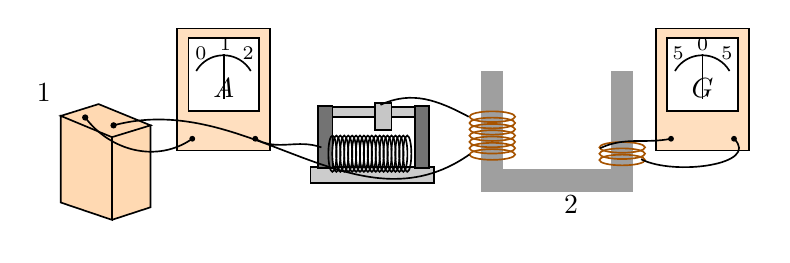
\begin{tikzpicture}[>=stealth,line width=.6pt]

\draw[fill=orange!30] (0,0)--(0,1.1)--(.65,.83)--(.65,-.22)--cycle (.65,.83)--(1.14,.98)--(1.14,-.06)--(.65,-.22) (0,1.1)--(.48,1.25)--(1.14,.98)--(.65,.83)--cycle;
\node[above left] at (0,1.16) {$1$};\fill(.31,1.08)circle(.04) (.67,.98)circle(.04);
\draw[fill=orange!25] (1.48,.66) rectangle (2.66,2.21) (7.56,.66) rectangle (8.74,2.21);
\foreach \x/\s in {2.07/A,8.15/G}{\draw[fill=white](\x-.45,1.16)rectangle(\x+.45,2.09);\draw(\x-.35,1.67) arc(150:30:.4);\draw(\x,1.32)--(\x,1.88);\node at(\x,1.45){$\s$};\fill(\x-.4,.81)circle(.037) (\x+.4,.81)circle(.037);}
\node at(1.78,1.9){\scriptsize $0$};\node at(2.09,2.01){\scriptsize $1$};\node at(2.38,1.9){\scriptsize $2$};
\node at(8.15,2.01){\scriptsize $0$};\node at(7.84,1.9){\scriptsize $5$};\node at(8.46,1.9){\scriptsize $5$};
\draw[fill=gray!40](3.17,.25)rectangle(4.74,.45) (3.29,1.09)rectangle(4.62,1.21);
\draw[fill=black!55](3.27,.44) rectangle(3.45,1.23) (4.5,.44)rectangle(4.68,1.23);
\foreach \x in {3.45,3.5,...,4.45}{\draw (\x,.62) ellipse(.052 and .23);}
\draw[fill=gray!45](3.99,.92) rectangle(4.2,1.26);
\draw[draw=gray!75,line width=8pt] (5.48,1.67)--(5.48,.28)--(7.13,.28)--(7.13,1.67);
\foreach \x/\y in {5.48/.61,5.48/.69,5.48/.77,5.48/.85,5.48/.93,5.48/1.01,5.48/1.09,7.13/.54,7.13/.62,7.13/.70}{\draw[orange!65!black] (\x,\y)ellipse(.29 and .068);}
\node[below] at(6.48,.22){$2$};
\draw(.31,1.08)to[out=-53,in=215](1.67,.81) (2.47,.81)to[out=-30,in=160](3.31,.7)
 (4.06,1.24)to[out=25,in=152](5.18,1.09) (5.19,.61)to[out=-145,in=15](.67,.98)
 (6.85,.69)to[out=25,in=191](7.75,.81) (7.37,.55)to[out=-27,in=-44](8.55,.81);

\end{tikzpicture}\end{center}

Как будут изменяться показания приборов при плавном уменьшении сопротивления реостата? Ответ поясните, указав, какие физические закономерности Вы использовали для объяснения.
}{
\smallskip\noindent\textbf{Решение}\par
$1$.  При плавном уменьшении сопротивления реостата ток в цепи будет плавно увеличиваться согласно закону Ома $I= \frac{U}{R} ,$ а значит, показания амперметра будут возрастать.
$2$.  Увеличение силы тока в цепи приведет к увеличению потока $\,\text{Ф}=LI$ вектора магнитной индукции через железный сердечник и, как следствие, приведет к возникновению небольшой ЭДС индукции $\mathcal E_{\,\text{инд}}$ в цепи этой катушки, $\mathcal E_{\,\text{инд}}\ll\mathcal E ,$ которой можно пренебречь.
$3$.  Увеличение потока вектора магнитной индукции через поперечное сечение сердечника вызовет изменение потока вектора индукции магнитного поля в проволочном мотке, соединенном с гальванометром. В соответствии с законом индукции Фарадея $\mathcal E_2= - \frac{\Delta \Phi}{\Delta t} ,$ что вызывает ток через гальванометр, вследствие чего стрелка гальванометра отклонится от начального положения.
}

% Source 41562: https://phys-ege.sdamgia.ru/problem?id=41562
\BankTask{41562}{
На фотографии представлена электрическая цепь. Начертите принципиальную схему этой электрической цепи. Опираясь на законы постоянного тока, объясните, как должны измениться (уменьшиться, увеличиться или остаться прежними) показания идеальных амперметра и вольтметра при замыкании ключа. Учесть внутреннее сопротивление батарейки, а сопротивлением подводящих проводов и ключа пренебречь.

\begin{center}\begin{tikzpicture}[>=stealth,line width=.6pt]

\draw[fill=orange!30] (0,0)--(0,.88)--(.7,.62)--(.7,-.25)--cycle (.7,.62)--(1.1,.8)--(1.1,-.07)--(.7,-.25) (0,.88)--(.43,1.07)--(1.1,.8)--(.7,.62)--cycle;
\fill(.24,.84)circle(.045) (.67,.82)circle(.045);
\foreach \x/\y/\value/\sign in {.75/2.05/{03{,}2}/V,3.15/.9/{00{,}6}/A}{
 \draw[fill=orange!35](\x-.61,\y-.42)rectangle(\x+.61,\y+.91);
 \draw[fill=white](\x-.43,\y+.01)rectangle(\x+.43,\y+.81);
 \node at(\x,\y+.57){$\value$};\node at(\x,\y+.22){$\sign$};
 \fill(\x-.42,\y-.25)circle(.055) (\x+.42,\y-.25)circle(.055);}
\draw[fill=gray!25](5.02,1.31)rectangle(6.84,1.57);
\fill(5.17,1.52)circle(.04) (6.58,1.52)circle(.04);
\draw[orange!65!black,line width=1.4pt](5.17,1.52)--(5.97,1.98);
\foreach \x/\r in {5.22/3,6.82/2}{
 \draw[fill=gray!20](\x-.57,.15)rectangle(\x+.58,.42);
 \foreach \i in {-.36,-.27,...,.36}{\draw(\x+\i,.45)ellipse(.095 and .095);}
 \fill(\x-.48,.32)circle(.04) (\x+.49,.32)circle(.04);
 \node at(\x,-.05){$\r\,\text{Ом}$};}
\draw(.24,.84) to[out=125,in=-155](.33,1.8) (.67,.82) to[out=52,in=-1](1.17,1.8)
 (.67,.82)to[out=-17,in=177](2.73,.65) (3.57,.65)to[out=-14,in=155](4.74,.32)
 (4.74,.32)to[out=110,in=180](5.17,1.52) (5.71,.32)to[out=30,in=60](6.34,.32)
 (5.71,.32)to[out=137,in=-65](6.58,1.52) (7.31,.32)to[out=-10,in=-31](.24,.84);

\end{tikzpicture}\end{center}
}{
\smallskip\noindent\textbf{Решение}\par
Схема электрической цепи имеет следующий вид: 

\begin{center}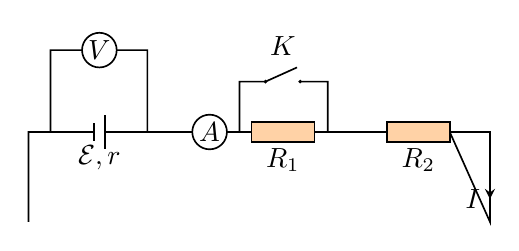
\begin{tikzpicture}[>=stealth,line width=.6pt]

\draw(0,0)--(0,1.14)--(.83,1.14) (.97,1.14)--(2.08,1.14) (2.52,1.14)--(2.83,1.14) (3.63,1.14)--(4.55,1.14) (5.35,1.14)--(5.86,1.14)--(5.86,0)--cycle
 (.28,1.14)--(.28,2.18)--(.68,2.18) (1.12,2.18)--(1.51,2.18)--(1.51,1.14)
 (2.68,1.14)--(2.68,1.78)--(3.01,1.78) (3.45,1.78)--(3.8,1.78)--(3.8,1.14);
\draw[->](5.86,.92)--(5.86,.29)node[left]{$I$};
\begin{scope}[shift={(0.9,1.14)},rotate=180]\draw(-.07,-.21)--(-.07,.21) (.07,-.11)--(.07,.11);\end{scope}\node[above right] at (1.02,1.14) {$$};\node[below] at(.9,1.1){$\mathcal E,r$};\draw (0.9,2.18)circle(.22) node {$V$};\draw (2.3,1.14)circle(.22) node {$A$};\begin{scope}[shift={(3.23,1.14)},rotate=0]\draw[fill=orange!35] (-.4,-.13) rectangle (.4,.13);\end{scope}\begin{scope}[shift={(4.95,1.14)},rotate=0]\draw[fill=orange!35] (-.4,-.13) rectangle (.4,.13);\end{scope}\node[below]at(3.23,1.06){$R_1$};\node[below]at(4.95,1.06){$R_2$};\begin{scope}[shift={(3.23,1.78)},rotate=0]\draw(-.22,0)--(.18,.18);\fill(-.22,0)circle(.025) (.22,0)circle(.025);\node[above]at(0,.2){$K$};\end{scope}
\end{tikzpicture}\end{center}

I  — сила тока в цепи.
При разомкнутом ключе ток будет проходить через резисторы R$_{1}$ и R$_{1}$, соединенные последовательно. Поэтому общее сопротивление цепи будет равно $R = R_1 + R_2.$
Амперметр измеряет общую силу тока в цепи, значение которой определяется законом Ома для полной цепи

\[I = \frac{\mathcal{E}}{R + r} ,\]

где $\mathcal{E}$  — ЭДС источника тока, r  — внутреннее сопротивление источника тока.
Исходя из закона Ома для участка цепи, содержащей последовательно соединенные резисторы, напряжение на внешней цепи, измеряемое вольтметром, U  =  IR. С учетом применения закона Ома для полной цепи данное напряжение равняется

\[U = \mathcal{E} - Ir.\]

Если замкнуть ключ, присоединенный параллельно к резистору R$_{1}$, то ток через данный резистор идти не будет. Поэтому общее сопротивление цепи станет равным R  =  R$_{2}$, а, следовательно, уменьшится. 
Из формулы закона Ома для полной цепи при уменьшении общего сопротивления сила тока в цепи увеличится. Напряжение соответственно формуле $U = \mathcal{E} - Ir.$ уменьшается.

Ответ: сила тока увеличивается, напряжение уменьшается.
}

% Source 11810: https://phys-ege.sdamgia.ru/problem?id=11810
\BankTask{11810}{
\begin{center}\begin{tikzpicture}[>=stealth,line width=.6pt]

\draw[task grid,step=.46] (0,0) grid (3.22,2.76);
\draw[task axis] (0,0)--(3.39,0) node[right] {$U,\,\text{В}$};
\draw[task axis] (0,0)--(0,2.93) node[above left] {$P,\,\text{Вт}$};
\foreach \x in {0,...,6}{\node[below] at (.46*\x,0) {$\x$};}
\foreach \y in {1,...,4}{\node[left] at (0,.46*\y) {$\y$};}
\draw[task curve,orange!85!black,domain=0:2.76,samples=80] plot(\x,{(2.3/1.9044)*\x*(2.76-\x)});

\end{tikzpicture}\end{center}
Электрическая цепь состоит из батареи с ЭДС \ensuremath{\mathcal E} и внутренним сопротивлением r и подключенного к ней резистора нагрузки с сопротивлением R. При изменении сопротивления нагрузки изменяется напряжение на ней и мощность в нагрузке. На рисунке представлен график зависимости мощности, выделяющейся на нагрузке, от напряжения на ней. Используя известные Вам физические законы, объясните, почему данный график зависимости мощности от напряжения представляет собой параболу.
}{
\smallskip\noindent\textbf{Решение}\par
Мощность, выделяющаяся на нагрузке вычисляется по формуле: $P = UI = \frac{U ^2}{R} .$ Сила тока по закону Ома для полной цепи равна $I = \frac{\mathcal{E}}{r + R} .$ Напряжение на нагрузке вычисляется по формуле $U = IR = \frac{\mathcal{E} R}{r + R} ,$ откуда $R = \frac{Ur}{\mathcal{E} - U} .$ Таким образом, получаем: $P = \frac{U ^2}{Ur} \cdot ( \mathcal{E} - U ) = \frac{U ( \mathcal{E} - U )}{r} .$ Данная функция является квадратичной функцией от напряжения, ее график  — парабола.
}

% Source 35341: https://phys-ege.sdamgia.ru/problem?id=35341
\BankTask{35341}{
\begin{center}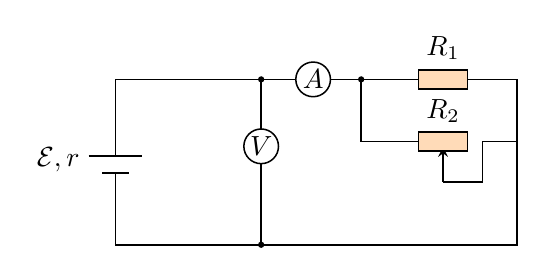
\begin{tikzpicture}[>=stealth,line width=.55pt]\draw(0,0)--(0,.91) (0,1.13)--(0,2.1)--(5.1,2.1)--(5.1,0)--(0,0);\draw(-.34,1.13)--(.34,1.13) (-.17,.91)--(.17,.91);\draw(1.85,0)--(1.85,2.1) (3.12,2.1)--(3.12,1.31)--(4.45,1.31);\fill(1.85,2.1)circle(.04) (1.85,0)circle(.04) (3.12,2.1)circle(.04);\draw[->](4.16,.8)--(4.16,1.24);\draw(4.16,.8)--(4.66,.8)--(4.66,1.31)--(5.1,1.31);\node[left]at(-.33,1.08){$\mathcal E,r$};\draw[fill=orange!28](3.85,1.98)rectangle(4.47,2.22);\node[above]at(4.16,2.22){$R_1$};\draw[fill=orange!28](3.85,1.19)rectangle(4.47,1.4300000000000002);\node[above]at(4.16,1.4300000000000002){$R_2$};\draw[fill=white](1.85,1.25)circle(.22)node{$V$};\draw[fill=white](2.51,2.1)circle(.22)node{$A$};\end{tikzpicture}\end{center}На рисунке показана принципиальная схема электрической цепи, состоящей из источника тока с отличным от нуля внутренним сопротивлением, резистора, реостата и измерительных приборов  — идеального амперметра и идеального вольтметра. Как будут изменяться показания приборов при перемещении движка реостата вправо? Ответ поясните, указав, какие физические закономерности Вы использовали для объяснения.
}{
\smallskip\noindent\textbf{Решение}\par
По условию задачи сопротивлением амперметра можно пренебречь, а сопротивление вольтметра бесконечно велико. При перемещении движка вправо сопротивление реостата R$_{2}$ увеличивается, что ведет к увеличению сопротивления R всей внешней цепи: $R= \frac{R_1 R_2}{R_1 + R_2} .$
В соответствии с законом Ома для полной цепи сила тока через амперметр уменьшается: $I= \frac{\mathcal{E}}{r + R}$ (знаменатель дроби растет, а числитель остается неизменным). Напряжение, измеряемое вольтметром, при этом растет: $U=I R=\mathcal{E} - I r.$

Ответ: напряжение, измеренное вольтметром, растет, а показания амперметра уменьшаются.
}

% Source 29734: https://phys-ege.sdamgia.ru/problem?id=29734
\BankTask{29734}{
\begin{center}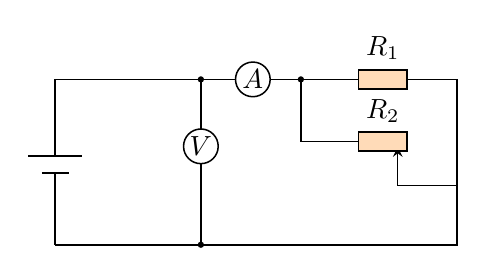
\begin{tikzpicture}[>=stealth,line width=.55pt]\draw(0,0)--(0,.91) (0,1.13)--(0,2.1)--(5.1,2.1)--(5.1,0)--(0,0);\draw(-.34,1.13)--(.34,1.13) (-.17,.91)--(.17,.91);\draw(1.85,0)--(1.85,2.1) (3.12,2.1)--(3.12,1.31)--(4.45,1.31);\fill(1.85,2.1)circle(.04) (1.85,0)circle(.04) (3.12,2.1)circle(.04);\draw[->](4.35,.75)--(4.35,1.24);\draw(4.35,.75)--(5.1,.75);\draw[fill=orange!28](3.85,1.98)rectangle(4.47,2.22);\node[above]at(4.16,2.22){$R_1$};\draw[fill=orange!28](3.85,1.19)rectangle(4.47,1.4300000000000002);\node[above]at(4.16,1.4300000000000002){$R_2$};\draw[fill=white](1.85,1.25)circle(.22)node{$V$};\draw[fill=white](2.51,2.1)circle(.22)node{$A$};\end{tikzpicture}\end{center} На рисунке изображена схема, содержащая источник тока с некоторым внутренним сопротивлением, резистор, реостат, амперметр и вольтметр. Как изменятся показания амперметра и вольтметра, если передвинуть ползунок реостата влево. Ответ поясните, указав, какие физические явления и закономерности Вы использовали для объяснения.
}{
\smallskip\noindent\textbf{Решение}\par
$1$.  При перемещении ползунка реостата влево происходит уменьшение длины проводника. Исходя из формулы для расчета сопротивления $R=\rho \frac{l}{S} ,$ делаем вывод, что сопротивление реостата $R_2$ уменьшается. 
$2$.  Реостат и резистор соединены между собой параллельно. Из формулы расчета общего сопротивления цепи $\frac{1}{R} = \frac{1}{R_1} + \frac{1}{R_2}$ следует, что общее сопротивление цепи также уменьшается. 
$3$.  По закону Ома для полной цепи $I= \frac{\mathcal{E}}{R + r}$ уменьшение общего сопротивления приведет к увеличению силы тока. Поскольку амперметр измеряет силу тока в неразветвленной части цепи, то его показания увеличатся. 
$4$.  Используя законы Ома для полной цепи и для участка цепи $I= \frac{U}{R} ,$ получаем, что $U=\mathcal{E} - I r.$ Увеличение силы тока приведет к уменьшению напряжения. Поскольку вольтметр измеряет напряжение на внешнем участке цепи, делаем вывод, что его показания уменьшаются. 

Ответ: показания амперметра увеличиваются, показания вольтметра уменьшаются.
}

% Source 41154: https://phys-ege.sdamgia.ru/problem?id=41154
\BankTask{41154}{
\begin{center}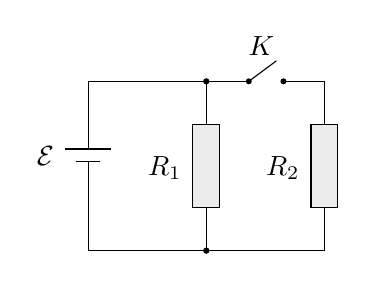
\begin{tikzpicture}[>=stealth]

\draw (0,0)--(3,0)--(3,.55) (3,1.6)--(3,2.15)--(2.48,2.15) (2.04,2.15)--(0,2.15)--(0,1.29) (0,1.13)--(0,0);
\draw (-.29,1.29)--(.29,1.29) (-.15,1.13)--(.15,1.13);
\node[left]at(-.31,1.2){$\mathcal E$};
\draw(1.5,0)--(1.5,.55) (1.5,1.6)--(1.5,2.15);
\draw(2.04,2.15)--(2.39,2.41);\node[above]at(2.2,2.35){$K$};
\fill(1.5,2.15)circle(.04) (1.5,0)circle(.04) (2.04,2.15)circle(.038) (2.48,2.15)circle(.038);
\draw[fill=gray!15] (1.33,.55)rectangle(1.67,1.6) (2.83,.55)rectangle(3.17,1.6);
\node[left]at(1.31,1.05){$R_1$};\node[left]at(2.81,1.05){$R_2$};
\end{tikzpicture}\end{center}
В электрической цепи, схема которой изображена на рисунке, ключ К сначала был разомкнут, а затем его замкнули. На сколько после этого изменилась тепловая мощность P, выделяющаяся в резисторе сопротивлением $R_{1}$  =  $10\,\text{Ом}$, если ЭДС батарейки равна $\mathcal E =12\,\text{В},$ её внутреннее сопротивление r  =  $2\,\text{Ом}$, а сопротивление резистора $R_{2}$  =  $15\,\text{Ом}$? Ответ дайте с учётом знака.
}{
\smallskip\noindent\textbf{Решение}\par
$1$.  До замыкания ключа К в левой части цепи по закону Ома для полной цепи течёт ток $I_1 = \frac{\mathcal E}{r + R_1} = 1\,\text{А},$ и в резисторе $R_{1}$ выделяется тепловая мощность $P_1 = I_1 ^2 R_1 = \frac{\mathcal E ^2 R_1}{( r + R_1 ) ^2} = 10\,\text{Вт}.$
$2$.  После замыкания ключа ток течёт уже через оба резистора $R_{1}$ и $R_{2}$. Согласно закону Ома для полной цепи, через батарейку течёт ток $I_2 = \frac{\mathcal E}{r + \frac{R_1R_2}{R_1 + R_2}} = 1{,}5\,\text{А}.$ При этом оба резистора $R_{1}$ и $R_{2}$ находятся под напряжением 

\[U_2 = \mathcal E - I_2r = \frac{\frac{ER_1R_2}{R_1 + R_2}}{r + \frac{R_1R_2}{R_1 + R_2}} = I_2 \frac{R_1R_2}{R_1 + R_2} .\]

$3$.  В резисторе $R_{1}$ при этом выделяется мощность 

\[P_2 = \frac{U_2 ^2}{R_1} = I_2 ^2 \frac{R_1R_2 ^2}{( R_1 + R_2 ) ^2} = 8{,}1\,\text{Вт}.\]

$4$.  Таким образом, изменение мощности после замыкания ключа равно: 

\[\Delta P = P_2 - P_1 = - 1{,}9\,\text{Вт}.\]

Ответ: $\Delta P = - 1{,}9\,\text{Вт}.$
}

% Source 16873: https://phys-ege.sdamgia.ru/problem?id=16873
\BankTask{16873}{
\begin{center}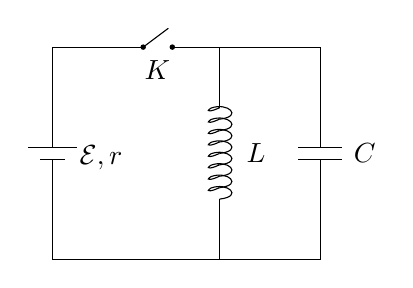
\begin{tikzpicture}[>=stealth]

\draw (0,0)--(3.4,0)--(3.4,1.27) (3.4,1.43)--(3.4,2.7)--(1.52,2.7) (1.15,2.7)--(0,2.7)--(0,1.43) (0,1.27)--(0,0)
(-.31,1.43)--(.31,1.43) (-.16,1.27)--(.16,1.27) (3.12,1.27)--(3.68,1.27) (3.12,1.43)--(3.68,1.43);
\draw(1.15,2.7)--(1.47,2.94);\fill (1.15,2.7)circle(.035) (1.52,2.7)circle(.035);
\node[below]at(1.33,2.65){$K$};\node[right]at(.22,1.30){$\mathcal E,r$};\node[right]at(3.7,1.35){$C$};
\draw (2.12,0)--(2.12,.77) (2.12,1.93)--(2.12,2.7);
\foreach \y in {.77,.915,1.06,1.205,1.35,1.495,1.64,1.785}{
 \begin{scope}[shift={(2.12,\y)}]\draw(0,0)..controls(.31,.035)and(.10,.22)..(-.11,.14)..controls(-.2,.08)and(-.08,.105)..(0,.145);\end{scope}}
\node[right]at(2.34,1.35){$L$};
\end{tikzpicture}\end{center}
В электрической цепи, показанной на рисунке, ключ К длительное время замкнут, $\mathcal E = 3\,\text{В},$ r = $2\,\text{Ом}$, L = $1$ мГн, С = $50$ мкФ. В момент t = $0$ ключ К размыкают. Каково напряжение U на конденсаторе в момент, когда в ходе возникших в контуре электромагнитных колебаний сила тока в контуре I = $1\,\text{А}$? Сопротивлением проводов и активным сопротивлением катушки индуктивности пренебречь.
}{
\smallskip\noindent\textbf{Решение}\par
Пока ключ замкнут через катушку течет постоянный ток $I_0,$ определяемый сопротивлением источника: $I_0 = \frac{\mathcal E}{r} .$ Поскольку активное сопротивление катушки, по условию, равно нулю, на катушке не падает напряжение, а значит, нулевое напряжение приложено к конденсатору. Таким образом, до размыкания ключа конденсатор разряжен. Начальная энергия электромагнитного поля в катушке $\frac{LI_0 ^2}{2} .$
После размыкания ключа начинаются электромагнитные колебания, и вся энергия, запасенная в катушке, будет перетекать из катушки в конденсатор и обратно. Энергия конденсатора равна $\frac{CU ^2}{2} .$ Через некоторое время энергия катушки уменьшится, а энергия конденсатора увеличится, причем сумма этих энергий будет равна начальной энергии катушки:

\[\frac{LI_0 ^2}{2} = \frac{LI ^2}{2} + \frac{CU ^2}{2} .\]

Откуда:

\[U = \sqrt{\frac{L ( I_0 ^2 - I ^2 )}{C}} = \sqrt{\frac{10^{-3} \,\text{Гн} \cdot \bigl( ( \frac{3\,\text{В}}{2\,\text{Ом}} ) ^2 - ( 1\,\text{А} ) ^2 \bigr)}{50 \cdot 10 ^{ - 6 } \,\text{Ф}}} = 5\,\text{В}.\]

Ответ: $5\,\text{В}$.
}

\end{document}
